\documentclass[twocolumn]{aastex631}
\usepackage{amsmath}
\usepackage{graphicx}
\usepackage{xcolor}
\graphicspath{{figures/}}
\newcommand{\vmac}{v_{\rm macro}}
\newcommand{\vsini}{v\sin i}
\newcommand{\teff}{T_{\rm eff}}
\newcommand{\nuchar}{\nu_{\rm char}}
\renewcommand{\ell}{\mathcal{L}}
\newcommand{\lgL}{\log\,\ell/\ell_\odot}
\newcommand{\lgLc}{\log\ell}
\newcommand{\lgT}{\log\,\teff}
\newcommand{\umag}{\mu{\rm mag}}
\newcommand{\dinv}{{\rm d}^{-1}}
\newcommand{\kms}{{\rm km\,s}^{-1}}
\newcommand{\todo}[1]{\textcolor{red}{[#1]}}

\shorttitle{Surface turbulence and red noise in massive stars}
\shortauthors{\todo{Authors}}

\begin{document}

\title{Surface turbulence and stochastic low-frequency variability in massive stars share a sub-surface driver}

\author{\todo{Author list}}
\affiliation{\todo{Affiliation}}

\begin{abstract}
Massive stars show ubiquitous stochastic low-frequency (SLF) photometric variability and broad, non-rotational spectral-line broadening (macroturbulence). Both have been attributed either to internal gravity waves (IGWs) excited by the convective core or to turbulence in sub-surface convection zones driven by the iron opacity bump (FeCZ). We assemble published red-noise fits for 486 OB and supergiant stars from eight studies and homogeneous macroturbulent velocities for 927 stars from the IACOB family of surveys, harmonize their units, place 342 red-noise and 832 macroturbulence stars on the spectroscopic HR diagram (sHRD; $\ell\equiv\teff^4/g$), and assign each a fractional main-sequence age $\tau$, mass, and radius from MIST tracks. On the homogeneous 196-star Galactic sample the red-noise amplitude $\alpha_0$ and $\vmac$ are organized by the same sHRD coordinate ($\alpha_0\propto\ell^{1.56\pm0.13}$, $\vmac\propto\ell^{0.29}$ at fixed $\teff$), whereas the characteristic frequency follows $\teff$ ($\nuchar\propto\teff^{1.53\pm0.34}$) and is flat in $\ell$. Gaussian-process posterior maps of all four quantities over the sHRD, weighted by an empirically measured 0.19-dex per-star systematic and a rotation penalty, make this two-coordinate structure explicit and extend it to red supergiants. Both $\vmac$ (hot stars) and $\alpha_0$ switch on at $\lgL\approx3.0$--3.2 ($\approx12\,M_\odot$ on the main sequence), above the luminosity at which one-dimensional models first develop an FeCZ, and $\vmac$ saturates at $\lgL\approx3.7$. At fixed mass, $\alpha_0$ grows by a factor of $\sim$50 from the zero-age to the terminal-age main sequence ($\partial\log\alpha_0/\partial\tau=+1.73^{+0.18}_{-0.17}$) while $\vmac$ grows by 1.9$\times$; the amplitude-to-velocity sensitivity ratio is $\approx5$--6 along both the luminosity and the age axis (but only $\approx2$ along the mass axis, where $\vmac$ responds strongly to mass). $\nuchar$ sits at $\sim$17 times the rotation frequency with no harmonic pile-up, but all three observables carry the same weak positive residual dependence on $\vsini$. Three-dimensional simulations of core-excited IGWs fall 3--4 orders of magnitude short of the observed amplitudes and predict none of these trends; a deepening, strengthening FeCZ predicts all of them. We conclude that sub-surface convection is the dominant driver of both phenomena in evolved OB stars, and identify the onset luminosity, the saturation luminosity, and the amplitude-to-velocity sensitivity ratios as quantitative targets for stellar-envelope models. The metallicity lever remains blocked by a fitting-method systematic between Galactic and Magellanic samples.
\end{abstract}

\keywords{Massive stars (732) --- Stellar convective zones (301) --- Stellar oscillations (1617) --- Stellar atmospheres (1584) --- Astrostatistics (1882)}

\section{Introduction}\label{sec:intro}

Space photometry has established that essentially every massive star varies stochastically at low frequencies \citep{bowman2019a,bowman2019b,bowman2020,burssens2020,bowman2023}. In the amplitude spectrum this appears as red noise, conventionally parameterized by a Lorentzian-like profile
\begin{equation}
A(\nu)=\frac{\alpha_0}{1+(\nu/\nuchar)^{\gamma}}+C_{\rm w},
\label{eq:lor}
\end{equation}
with an amplitude at zero frequency $\alpha_0$, a characteristic frequency $\nuchar$ at which the spectrum turns over, a high-frequency slope $\gamma$, and a white-noise floor $C_{\rm w}$. High-resolution spectroscopy has, in parallel, shown that the photospheric line profiles of O and B stars require a non-rotational broadening component of tens of $\kms$---macroturbulence, $\vmac$---that is supersonic, ubiquitous above a certain luminosity, and organized in the Hertzsprung--Russell diagram \citep{simondiaz2010,simondiaz2014,simondiaz2017}.

Two physical pictures compete to explain one or both phenomena. In the first, internal gravity waves (IGWs) excited at the boundary of the convective core propagate through the radiative envelope and reach the surface, where their superposition produces both a stochastic photometric signal \citep{rogers2013,aerts2015,edelmann2019,ratnasingam2020} and a collective tangential velocity field that broadens lines \citep{aerts2009}. In the second, the iron-opacity bump drives a thin sub-surface convection zone (FeCZ) whose turbulent motions, and the waves they launch, produce the surface velocity field and the photometric variability directly \citep{cantiello2009,grassitelli2015,cantiello2021,schultz2022,jermyn2022}.

The two pictures make different predictions for how the observables should scale with position on the HR diagram and with evolution. In the FeCZ picture the convective flux, and hence both $\alpha_0$ and $\vmac$, should track the envelope's proximity to the Eddington limit, which on the spectroscopic HR diagram (sHRD) is the ordinate $\ell\equiv\teff^4/g\propto L/M$ \citep{cantiello2021}. The turnover frequency should track the convective turnover time, which is set by local envelope conditions and depends chiefly on $\teff$. The FeCZ does not exist below a threshold luminosity at solar metallicity, so both signals should switch on rather than fade in. Because the FeCZ deepens and strengthens as the envelope expands along the main sequence, amplitudes should grow with fractional main-sequence age at fixed mass. In the core-IGW picture, by contrast, the wave flux is set by the convective core; amplitude grows slowly with mass, the surface spectrum is expected to soften and shift to lower frequency as the envelope thickens and damping increases, and three-dimensional simulations predict surface amplitudes of order 0.1~$\umag$ for a 15~$M_\odot$ star \citep{anders2023}---orders of magnitude below what is observed.

Existing tests have used samples of a few tens to $\sim$100 stars \citep{bowman2020,bowman2022,bowman2024,ma2024,shen2024}. They established that $\nuchar$ correlates with position in the sHRD and that the phenomenon persists to Small Magellanic Cloud metallicity, but each sample alone lacks the dynamic range in luminosity, temperature, and evolutionary state to discriminate between the two pictures on functional form rather than on the sign of a correlation. Here we combine every published red-noise sample we could locate with the full IACOB macroturbulence database, harmonize them, and ask three quantitative questions: (1) Are $\alpha_0$, $\nuchar$, $\gamma$, and $\vmac$ organized by the same coordinates on the sHRD? (2) Is there a luminosity onset, and where is it relative to the predicted appearance of the FeCZ? (3) How do the observables evolve along the main sequence at fixed mass, and does rotation act as a clock or as a modifier?

Section~\ref{sec:data} describes the samples and their harmonization; Section~\ref{sec:methods} the statistical methods; Section~\ref{sec:results} the results; Section~\ref{sec:discussion} confronts them with theory, and Section~\ref{sec:conclusions} summarizes.

\section{Data}\label{sec:data}

\subsection{Red-noise samples}\label{sec:rednoise}

We compiled every published table of Lorentzian or Gaussian-process (GP) red-noise fits to space photometry of OB and supergiant stars that we could locate through a keyword search of the VizieR table metadata (via TAP/ADQL, searching table descriptions for ``stochastic low-frequency'', ``red noise'', and author names), supplemented by tables transcribed from the papers themselves. The result is 486 stars from eight sources (Table~\ref{tab:samples}): the Galactic TESS samples of \citet[70 stars]{bowman2020} and \citet[150 stars, of which 126 are not in Bowman et al.]{shen2024}; the K2 and LMC TESS samples of \citet{bowman2019b}; the LMC and SMC GP-regression samples of \citet{bowman2024}; the LMC blue supergiants of \citet{ma2024}; the Galactic yellow and red supergiants of \citet{dornwallenstein2020}; and the CoRoT sample of \citet{bowman2019a}. The CoRoT and K2 stars lack the spectroscopic parameters needed for the sHRD and are retained in the catalog but not used in the analysis below.

For the two Galactic TESS samples, which share the same Lorentzian parameterization and the same units ($\alpha_0$ in $\umag$, $\nuchar$ in $\dinv$), we verified the compatibility of the fits directly: 24 stars were fitted independently by both studies. The offsets are negligible (median $\Delta\log\alpha_0=+0.03$~dex, $\Delta\log\nuchar=-0.06$~dex) and the correlations strong (Spearman $\rho=0.93$ and 0.69; Figure~\ref{fig:overlap}). The scatter about the identity, 0.19~dex in both $\log\alpha_0$ and $\log\nuchar$ and 0.39 in $\gamma$, is the empirical per-star systematic uncertainty of a red-noise fit and is used as the error floor throughout (Section~\ref{sec:weights}). The published formal uncertainties, which we confirmed from the CDS ReadMe to be in $\umag$, are $10^{-5}$--$10^{-2}$ relative and represent MCMC statistical errors on a well-sampled spectrum; they are two orders of magnitude smaller than the measured study-to-study scatter and are not used. The union of the two studies (196 stars) forms the \emph{primary homogeneous Galactic sample} on which all amplitude scaling relations are derived. Shen et al.\ report per-sector fits; we take the median across sectors.

\subsection{Macroturbulence samples}\label{sec:vmac}

Macroturbulent velocities come from the IACOB project and its associated analyses \citep{simondiaz2014,simondiaz2017,holgado2018,deburgos2023,deburgos2024,burssens2020}, all of which measure a radial--tangential macroturbulent broadening together with $\vsini$ from a Fourier-transform plus goodness-of-fit analysis of metal lines. Where a star appears in more than one source we adopt the value from the first in the priority order of Table~\ref{tab:vmac}; the sources agree pairwise to a median offset of $\lesssim1~\kms$ with rank correlations of 0.70--0.88. The unified catalog contains 927 stars, 832 of which have the $\teff$ and $\log g$ needed for the sHRD.

\citet{shen2024} also tabulate a broadening velocity labelled ``vmacro''. Against the IACOB values for the 69 stars in common it is offset by $-18$ to $-25~\kms$ with rank correlation $\rho\le0.5$; 32\% of its values exceed 150~$\kms$ (versus 0.4\% in IACOB) and 32 stars have a ``vmacro'' but no $\vsini$. We interpret this column as a single total-broadening parameter in which rotation has been absorbed and exclude it; Shen et al.'s red-noise parameters and atmospheric parameters, which validate against Bowman et al.\ as described above, are retained.

\subsection{Harmonization}\label{sec:harmon}

All $\nuchar$ values are expressed in $\dinv$ (the CoRoT values were converted from $\mu$Hz). The amplitude $\alpha_0$ is published in four mutually incompatible conventions across the samples: an amplitude in $\umag$ (Bowman et al.\ 2020; Shen et al.), an amplitude in ppm of unconfirmed normalization (Bowman et al.\ 2019b; Ma et al.), a power-spectral-density maximum in mmag$^2\,{\rm d}$ (Bowman et al.\ 2024), and a PSD in ppm$^2\,\mu{\rm Hz}^{-1}$ (Bowman et al.\ 2019a). \citet{dornwallenstein2020} use a different functional form (a damped random walk parameterized by a timescale) and tabulate an amplitude whose unit we could not confirm from the catalog metadata. Amplitudes enter the analysis at two levels. The scaling coefficients of Table~\ref{tab:fits} use only the 196 $\umag$ amplitudes of the primary sample. The sHRD amplitude map and the onset test additionally include the 26 ppm amplitudes of \citet{bowman2019b} and \citet{ma2024} (1~ppm $=1.086~\umag$, a $\le0.04$-dex offset that is negligible against the 0.19-dex floor and is absorbed into an added systematic of 0.05 and 0.15~dex respectively, the latter reflecting Ma et al.'s modified Lorentzian form); these 222 stars are those flagged as amplitude-compatible in the machine-readable table. The PSD-proxy and Dorn-Wallenstein amplitudes are never used; those samples contribute $\nuchar$ and $\gamma$ only. Dorn-Wallenstein et al.'s timescale $\tau_{\rm DW}$ was converted to $\nuchar=1/(2\pi\tau_{\rm DW})$.

Luminosities are of two kinds. The spectroscopic luminosity $\ell\equiv\teff^4/g$ \citep{langer2014}, normalized with $\ell_\odot=(5777\,{\rm K})^4/(274\,{\rm m\,s^{-2}}\times100)$, requires only $\teff$ and $\log g$ and is the quantity on which FeCZ properties depend \citep{cantiello2021}. The IACOB sources publish $\ell$ directly (we verified that Shen et al.'s tabulated $\log\ell$ reproduces this definition to $<0.005$~dex). The Magellanic and supergiant red-noise samples publish only the classical bolometric luminosity, without $\log g$. One correction was required: \citet{holgado2018} tabulate $\teff$ in kK, and the affected 62 stars were re-derived.

\subsection{Placing stars on the spectroscopic HR diagram}\label{sec:shrd}

For the 146 red-noise stars without a published $\log g$ we used two routes. \textbf{Tier A} (47 stars): we located the parent spectroscopic analyses of the Magellanic samples---\citet{bestenlehner2025}, \citet{vink2023}, \citet{urbaneja2017}, and \citet{mcevoy2015}---and matched by name (after normalizing designations) and by position within $2''$. Urbaneja et al.\ publish the flux-weighted gravity $\log g_F=\log g-4\log(\teff/10^4\,{\rm K})$, which we inverted. The matched $\teff$ agree with those used by the red-noise papers to a median of 0.000~dex (MAD 0.005), confirming that these are the same parameter sources. \textbf{Tier B} (99 stars, including all Dorn-Wallenstein et al.\ supergiants): because $\ell/\ell_\odot=(L/L_\odot)/(M/M_\odot)$ exactly, a classical luminosity and a mass suffice. We estimated the mass from the nearest point on the MIST v1.2 solar-metallicity, $v/v_{\rm crit}=0.4$ tracks \citep{choi2016,dotter2016} in the $(\lgT,\log L)$ plane, weighting the eight nearest track points by inverse squared distance. Calibrating on the 33 Magellanic stars that have both routes gives a tier-B offset of $-0.09$~dex and a scatter of 0.19~dex (Figure~\ref{fig:tierB}); the offset is applied and the scatter propagated into the weights through each property's sHRD gradient (Section~\ref{sec:weights}). The final sHRD sample comprises 342 red-noise stars (243 tier A, 99 tier B) spanning $\lgT=3.53$--4.76 and $\lgL=2.33$--4.58 (Figure~\ref{fig:samples}).

\subsection{Evolutionary parameters}\label{sec:evol}

Every star on the sHRD was assigned a fractional main-sequence age $\tau$ (0 at the ZAMS, 1 at the TAMS, $>1$ beyond), a current mass, and a radius from the nearest MIST track point in $(\lgT,\lgL)$, using the same distance-weighted scheme. Validated against the independently derived values that \citet{shen2024} publish for 126 stars, our track-based masses agree to a median $\Delta\log M=0.00$ (MAD 0.02~dex) and our $\tau$ to a median offset of $+0.08$ (MAD 0.04), the offset reflecting the different input physics of their tracks. The projected rotation frequency $f_{\rm rot}=\vsini/(2\pi R)$, a lower limit on the true rotation frequency, follows from the track radius. Stars whose nearest track point lies more than 0.5 (in the scaled metric) from any track are flagged and excluded from the evolutionary analyses (9 of 342).

\section{Methods}\label{sec:methods}

\subsection{Correlations, model selection, and uncertainties}\label{sec:stats}

Univariate dependences are quantified with Spearman rank correlations. Multivariate power laws are fitted as linear models in log space; because $\lgL=4\lgT-\log g-{\rm const}$ is an identity, $\ell$, $\teff$, and $\log g$ cannot enter the same model and we use the $\{\ell,\teff\}$ basis throughout (variance-inflation factors $<2.5$). Over the 126 stars with all three published, the identity holds to a median of 0.0005~dex (MAD 0.003); the four stars that deviate by $>0.1$~dex ($\theta^1$~Ori~C, HD~108, HD~191612, HD~15137) are known magnetic or binary objects whose parameters were assembled from different analyses. Predictor sets are selected by the Bayesian information criterion over all subsets, and coefficient intervals are 16--84\% ranges from 3000--5000 bootstrap resamples.

\subsection{Reliability weights}\label{sec:weights}

For the sHRD maps each star $i$ receives a variance $\sigma_i^2=\sigma_{\rm sys}^2+\sigma_{{\rm rot},i}^2+\sigma_{{\rm B},i}^2$. The first term is the study-to-study systematic of Section~\ref{sec:rednoise} (0.186~dex for $\log\alpha_0$, 0.192~dex for $\log\nuchar$, 0.39 for $\gamma$) or, for $\vmac$, the $\sim$20\% pairwise scatter between IACOB sources (0.08~dex). The second addresses the degeneracy between rotational and macroturbulent broadening and the difficulty of separating rotational modulation from red noise in rapid rotators:
\begin{equation}
\sigma_{{\rm rot},i}=0.35\,\frac{\vsini_i}{\vsini_i+100~\kms}~{\rm dex},
\end{equation}
which reaches 0.18~dex at $\vsini=100~\kms$ and 0.26~dex at 300~$\kms$; stars without a $\vsini$ measurement receive the midpoint penalty of 0.175~dex. The third applies to tier-B stars only and propagates the 0.19-dex placement scatter through each property's fitted sHRD gradient. The maps are insensitive to the rotation term: removing it changes the posterior mean by a median of $<0.02$~dex over the trustworthy region for every property.

\subsection{Gaussian-process maps and their trustworthy region}\label{sec:gp}

The expected value of each property as a function of sHRD position was obtained by GP regression with a constant-times-Mat\'ern($\nu=5/2$) kernel with independent length scales in $\lgT$ and $\lgL$, the per-star variances $\sigma_i^2$ entering as heteroscedastic noise, inputs and targets standardized, and hyperparameters set by marginal-likelihood maximization with four restarts. The posterior standard deviation of the latent mean quantifies interpolation uncertainty but does not by itself flag extrapolation: a smooth field extrapolates confidently into regions containing no stars. A grid point is therefore marked trustworthy only if the posterior s.d.\ is below 0.6 times the property's overall scatter \emph{and} at least three stars lie within an ellipse of semi-axes 0.06 in $\lgT$ and 0.25 in $\lgL$. Two grids are used: an OB grid ($\lgT=4.03$--4.72) for $\vmac$ and $\alpha_0$, which have no data cooler than that, and an extended grid ($\lgT=3.50$--4.78) for $\nuchar$ and $\gamma$.

\subsection{Onset test}\label{sec:onset_method}

To test for a luminosity threshold we compare, for each observable, a single power law in $\ell$ against a continuous broken power law with a free hinge $h$, both with $\lgT$ as a covariate so that a temperature mix along the $\ell$ axis cannot masquerade as a break:
\begin{align}
\log(\cdot)={}&c_0+c_1(\lgLc-h)\nonumber\\
&+c_2\max(0,\lgLc-h)+c_3\lgT.
\end{align}
The hinge is scanned on a 0.02-dex grid with at least ten stars on each side; the interval on $h$ comes from 300 bootstrap resamples. A break is claimed only for $\Delta{\rm BIC}>6$ with the hinge interior to the grid.

\subsection{Rotation test}\label{sec:rot_method}

If the red-noise turnover were rotational modulation, $\nuchar$ would sit at $f_{\rm rot}$ or its first harmonic and the distribution of $\log(\nuchar/f_{\rm rot})$ would pile up near 0 or $\log2$. If rotation instead modifies the underlying driver, $\nuchar$, $\alpha_0$, and $\vmac$ should each carry a smooth residual dependence on $\vsini$ after $\ell$ and $\teff$ are removed. We test both, the second via added-variable (partial-residual) regressions. Because $\vsini$ is a lower limit on the equatorial velocity, and because the rotation--macroturbulence fitting degeneracy would produce an \emph{anti}-correlation between $\vmac$ and $\vsini$, a positive residual slope for $\vmac$ is conservative.

\section{Results}\label{sec:results}

\begin{figure*}
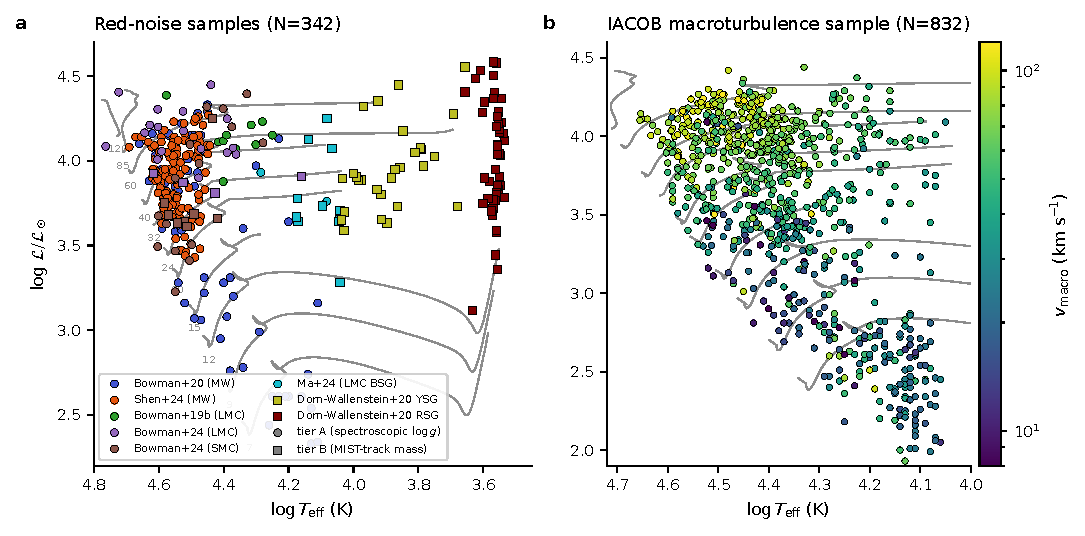
\includegraphics[width=\textwidth]{fig1_samples.pdf}
\caption{The compiled samples on the spectroscopic HR diagram. (a) The 342 red-noise stars, colored by source; circles are tier-A placements (spectroscopic $\log g$), squares tier-B (MIST-track mass). (b) The 832 IACOB stars with macroturbulent velocities, colored by $\vmac$. Grey curves are MIST v1.2 solar-metallicity tracks labelled by initial mass in $M_\odot$.}
\label{fig:samples}
\end{figure*}

\begin{figure*}
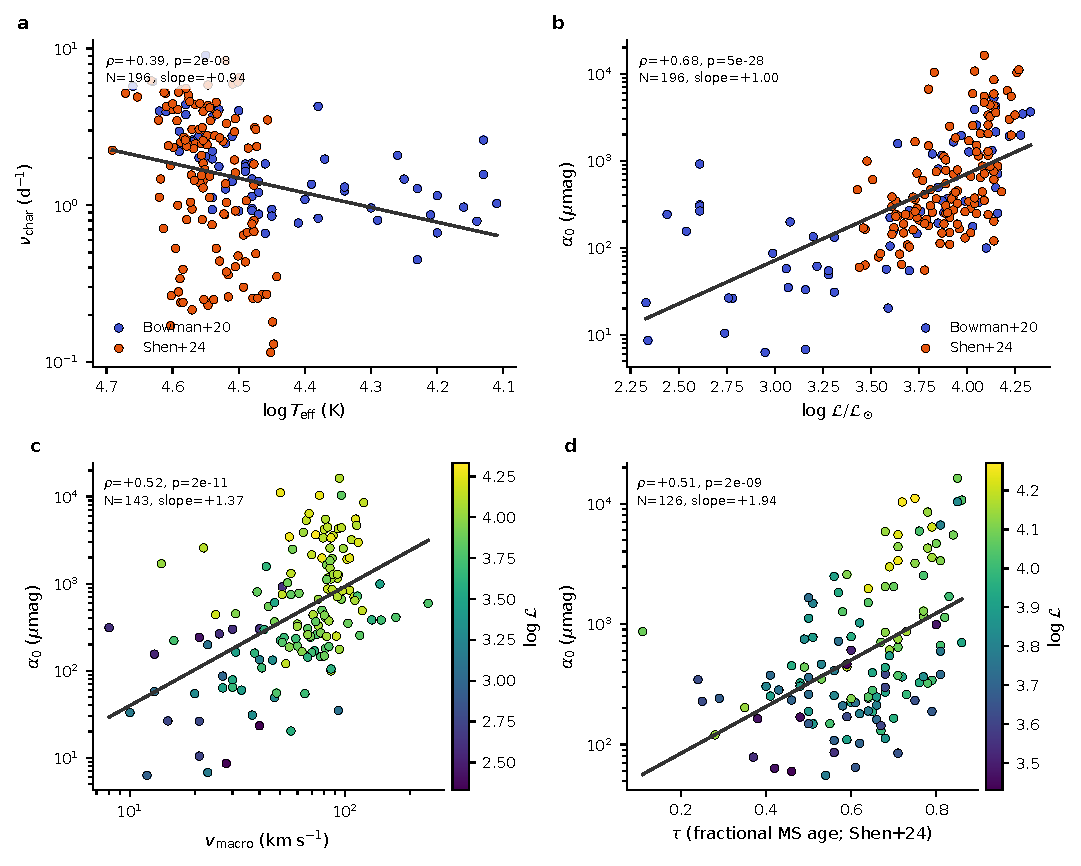
\includegraphics[width=\textwidth]{fig2_scalings.pdf}
\caption{Scaling relations on the primary homogeneous Galactic sample (Bowman et al.\ 2020 $\cup$ Shen et al.\ 2024, $N=196$). (a) $\nuchar$ against $\teff$; (b) $\alpha_0$ against spectroscopic luminosity; (c) $\alpha_0$ against IACOB macroturbulence, colored by $\lgL$; (d) $\alpha_0$ against the fractional main-sequence age published by Shen et al. Lines are least-squares power laws; the Spearman coefficient, sample size, and slope are given in each panel.}
\label{fig:scalings}
\end{figure*}

\subsection{Two orthogonal coordinates on the sHRD}\label{sec:coords}

On the primary sample, the red-noise amplitude and the characteristic frequency depend on different sHRD coordinates (Figure~\ref{fig:scalings}; Table~\ref{tab:fits}). The BIC-preferred model for the amplitude is
\begin{align}
\log\alpha_0 = 1.56^{+0.12}_{-0.13}\,\lgLc - 3.16^{+0.62}_{-0.66}\,\lgT + c
\end{align}
($R^2=0.53$), i.e.\ $\alpha_0$ rises steeply with $\ell$ and, at fixed $\ell$, is lower in hotter stars. For the characteristic frequency,
\begin{equation}
\log\nuchar = 1.53^{+0.35}_{-0.33}\,\lgT - 0.23^{+0.09}_{-0.09}\,\lgLc + c
\end{equation}
($R^2=0.09$): $\nuchar$ rises with $\teff$ and is nearly flat in $\ell$. The univariate correlation of $\nuchar$ with $\ell$ is null ($\rho=-0.02$), that of $\alpha_0$ with $\teff$ is null ($\rho=-0.09$; Figure~\ref{fig:corr}). Both quantities correlate with $\vsini$ ($\rho=+0.24$ and $+0.32$), $\alpha_0$ correlates with $\log g$ ($\rho=-0.64$), with $\vmac$ ($\rho=+0.52$, $N=144$), and with Shen et al.'s fractional age and mass ($\rho=+0.51$ each), while $\gamma$ correlates with nothing but $\vsini$ ($\rho=+0.17$). The slope $\gamma$ is nearly universal: its 16--84\% range on the primary sample is 1.43--2.45 with median 1.91.

The macroturbulent velocity, fitted over the full IACOB sample in the same way, follows the amplitude rather than the frequency: $\partial\log\vmac/\partial\lgL=+0.29$, $\partial\log\vmac/\partial\lgT=+0.10$ ($N=832$, $R^2=0.44$). Thus $\alpha_0$ and $\vmac$ share the $\ell$ coordinate while $\nuchar$ is set by $\teff$, and $\alpha_0$ is about five times more sensitive to $\ell$ than $\vmac$ is.

\begin{figure*}
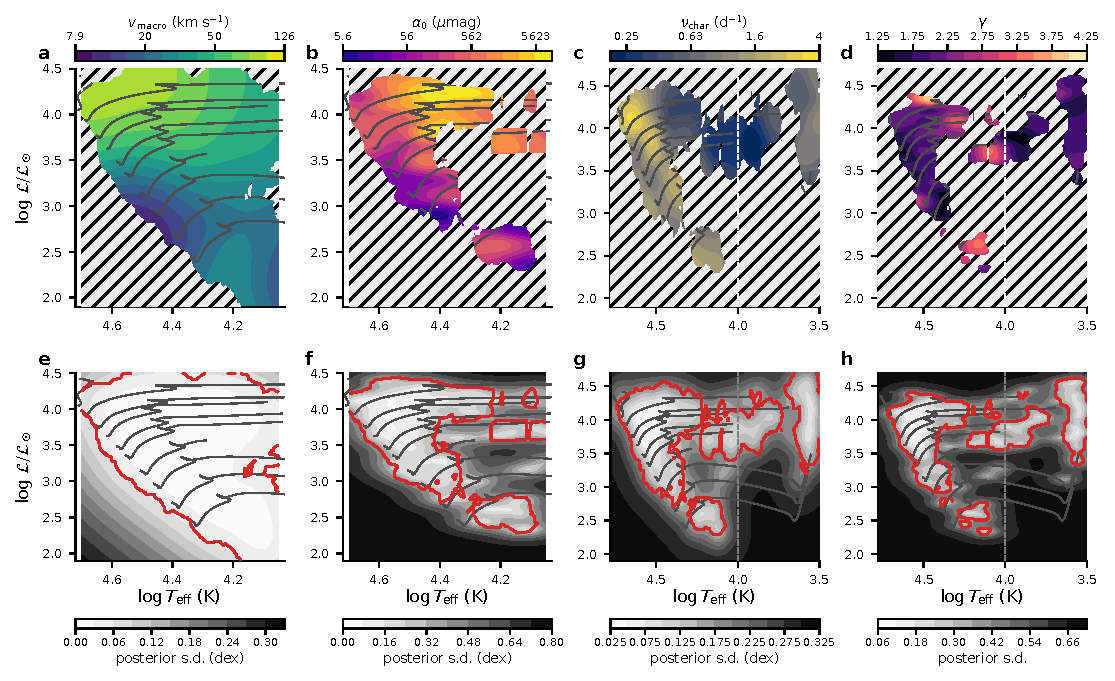
\includegraphics[width=\textwidth]{fig3_gpmaps.pdf}
\caption{Expected value of each property at every position on the sHRD, from reliability-weighted Gaussian-process regression (top row), and the posterior standard deviation of the latent mean (bottom row). Hatched grey regions fail the trustworthiness criterion (posterior s.d.\ below 0.6 of the property's scatter \emph{and} at least three stars within a local ellipse); the red contour in the bottom row bounds the trustworthy region. $\vmac$ and $\alpha_0$ use an OB grid; $\nuchar$ and $\gamma$ an extended grid reaching the red supergiants (the dashed line marks $\lgT=4.0$). Black curves are MIST tracks.}
\label{fig:gpmaps}
\end{figure*}

The GP maps (Figure~\ref{fig:gpmaps}) show the same structure without any parametric assumption. Iso-contours of $\vmac$ and of $\alpha_0$ run nearly horizontally---both properties increase upward along $\ell$ and are almost blind to $\teff$ at fixed $\ell$---whereas iso-contours of $\nuchar$ run nearly vertically across the OB region, decreasing toward cooler temperatures. The fitted GP length scales are diagnostic in themselves: for $\vmac$ they are long in both coordinates (a smooth field); for $\nuchar$ the $\ell$ length scale runs to the upper bound (no $\ell$ dependence at all); for $\gamma$ the map is patchy, with correlation lengths comparable to the inter-star spacing, meaning the field carries little structure beyond noise.

\subsection{A luminosity onset above the FeCZ threshold}\label{sec:onset}

\begin{figure*}
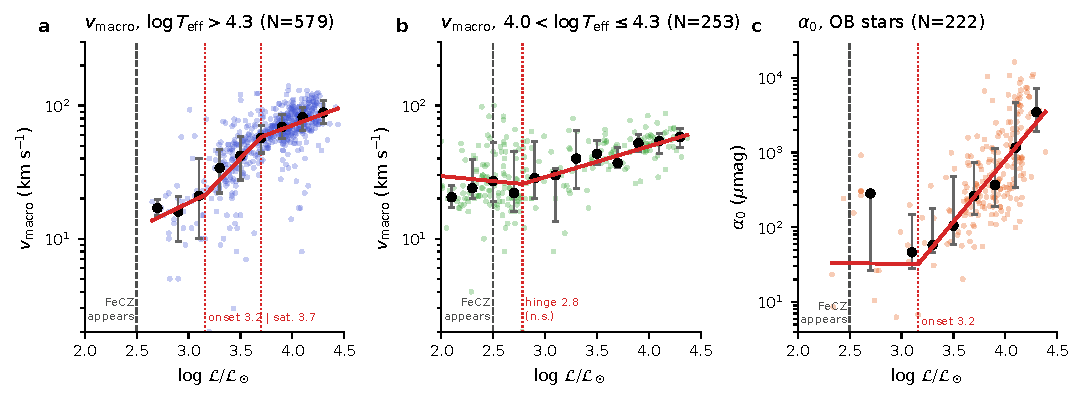
\includegraphics[width=\textwidth]{fig4_onset.pdf}
\caption{Broken-power-law test for a luminosity onset, with $\lgT$ as a covariate. (a) IACOB $\vmac$ for stars hotter than $\lgT=4.3$; (b) IACOB $\vmac$ for $4.0<\lgT\le4.3$; (c) red-noise amplitude for OB stars. Faint points are individual stars, black points binned medians with 16--84\% ranges, red curves the best broken fit evaluated at the median $\teff$, dotted red lines the hinge positions, and the dashed grey line the luminosity at which solar-metallicity models first develop an iron convection zone \citep{cantiello2009,cantiello2021}.}
\label{fig:onset}
\end{figure*}

Table~\ref{tab:onset} and Figure~\ref{fig:onset} summarize the onset test. For the hot IACOB stars ($\lgT>4.3$, $N=579$) a break is strongly preferred ($\Delta{\rm BIC}=+15$), and a second hinge is preferred over one by a further $\Delta{\rm BIC}=17.5$: $\vmac$ sits on a floor of $\approx16~\kms$ below $\lgL=3.16$, rises as $\ell^{0.81}$ between 3.16 and 3.70, and flattens to $\ell^{0.29}$ above 3.70. The red-noise amplitude of OB stars ($N=222$) shows an onset at the same place, $\lgL=3.16$ [2.94, 3.44] ($\Delta{\rm BIC}=+16$): flat below ($-0.02$), rising as $\ell^{1.66}$ above. Only 19 stars lie below the hinge, and their amplitudes are bimodal (a handful near 300~$\umag$, the rest at $\sim$30~$\umag$), so the sub-onset level is poorly constrained. In the cooler B-star band ($4.0<\lgT\le4.3$, $N=253$) $\vmac$ rises only gently and monotonically with $\ell$ and the break test is inconclusive ($\Delta{\rm BIC}=+4.8$). $\nuchar$ shows no break ($\Delta{\rm BIC}=-0.6$).

On the MIST tracks, $\lgL=3.16$ at $\lgT>4.3$ corresponds to main-sequence stars of $\approx12\,M_\odot$ and $\log L/L_\odot\approx4.0$. One-dimensional models at solar metallicity first develop an FeCZ at $\lgL\approx2.5$ \citep{cantiello2009,cantiello2021}, 0.6~dex below the observed onset.

\subsection{Evolution along the main sequence at fixed mass}\label{sec:evolution}

\begin{figure*}
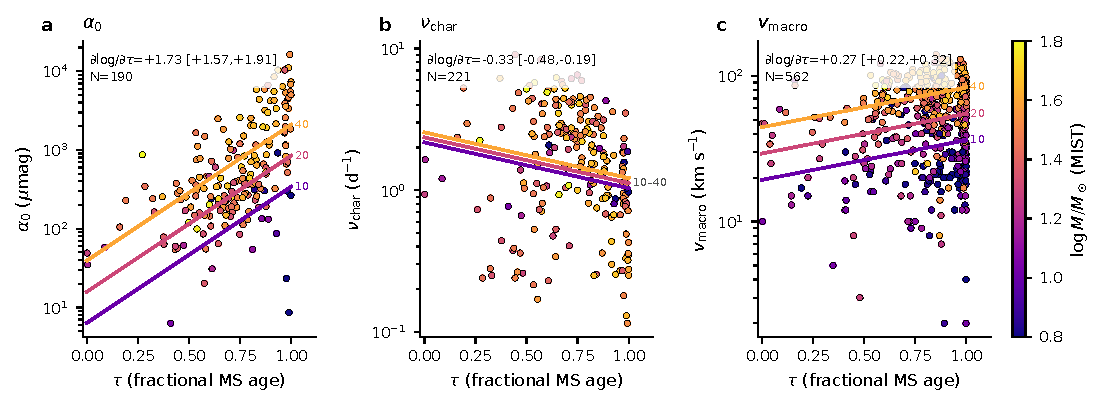
\includegraphics[width=\textwidth]{fig5_evolution.pdf}
\caption{Evolution along the main sequence at fixed mass. Each star is placed at its MIST-derived fractional main-sequence age $\tau$ and colored by MIST mass; lines show the fitted model $\log(\cdot)=a\tau+b\log M$ at 10, 20, and 40~$M_\odot$. (a) $\alpha_0$ on the primary sample ($N=190$); (b) $\nuchar$ on all OB stars with $\tau<1$ ($N=221$; the three mass lines coincide); (c) IACOB $\vmac$ ($N=562$).}
\label{fig:evolution}
\end{figure*}

Restricting to well-placed main-sequence stars ($\tau<1$) and fitting $\log(\cdot)=a\,\tau+b\,\log M$ (Table~\ref{tab:fits}; Figure~\ref{fig:evolution}): the red-noise amplitude grows as
\begin{align}
\partial\log\alpha_0/\partial\tau&=+1.73^{+0.18}_{-0.17},\\
\partial\log\alpha_0/\partial\log M&=+1.32^{+0.20}_{-0.21}
\end{align}
($N=190$, $R^2=0.51$)---a factor of $\sim$50 from ZAMS to TAMS at fixed mass. Macroturbulence grows as $\partial\log\vmac/\partial\tau=+0.27^{+0.05}_{-0.05}$ ($\times1.9$ across the main sequence) with $\partial\log\vmac/\partial\log M=+0.60\pm0.03$ ($N=562$, $R^2=0.45$). The characteristic frequency declines slowly, $\partial\log\nuchar/\partial\tau=-0.33^{+0.14}_{-0.15}$, with almost no mass dependence ($+0.12$) and $R^2=0.03$. The same model fitted on the 126 Shen et al.\ stars with their own published $\tau$ and $M$ gives $\partial\log\alpha_0/\partial\tau=+1.91$ and $\partial\log\alpha_0/\partial\log M=+1.83$; the difference in the mass coefficient reflects the larger dynamic range in mass of the full sample and the different track physics. Beyond the TAMS the growth stops: the 28 post-main-sequence OB stars with $\umag$ amplitudes have median $\alpha_0=877~\umag$ against 1211~$\umag$ for the 82 main-sequence stars with $\tau>0.8$ (Mann--Whitney $p=0.22$).

The amplitude-to-velocity sensitivity ratio $(\partial\log\alpha_0/\partial x)/(\partial\log\vmac/\partial x)$ is $5.3$ for $x=\lgL$, $6.4$ for $x=\tau$, and $2.2$ for $x=\log M$; on the 144-star subsample with both quantities the direct power law is $\alpha_0\propto\vmac^{1.37}$ (Figure~\ref{fig:scalings}c).

\subsection{Rotation: not the clock, but a common modifier}\label{sec:rotation}

\begin{figure*}
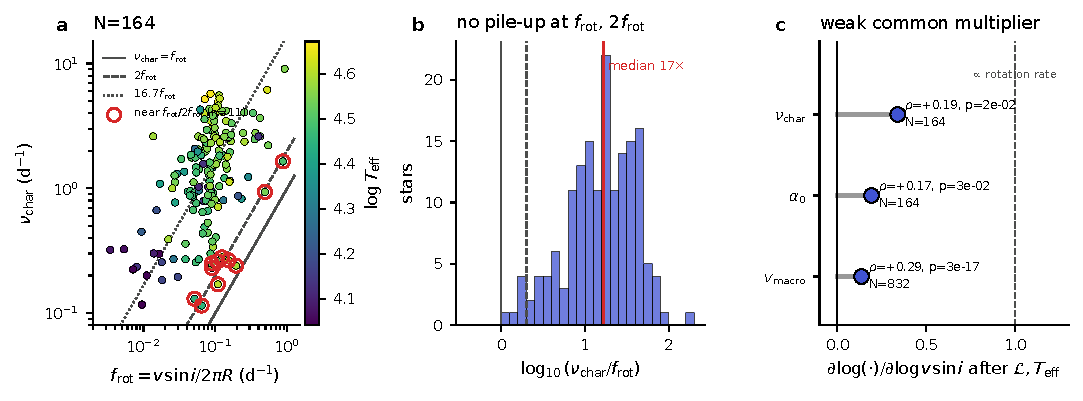
\includegraphics[width=\textwidth]{fig6_rotation.pdf}
\caption{Rotation test on the 164 OB stars with $\vsini$, $\nuchar$, and a MIST radius. (a) $\nuchar$ against the projected rotation frequency $f_{\rm rot}=\vsini/2\pi R$; lines mark $\nuchar=f_{\rm rot}$, $2f_{\rm rot}$, and the sample median ratio $16.7\,f_{\rm rot}$; red circles are the 11 stars within 0.15~dex of $f_{\rm rot}$ or $2f_{\rm rot}$. (b) Distribution of $\log(\nuchar/f_{\rm rot})$. (c) Residual slope of each observable against $\log\vsini$ after $\ell$ and $\teff$ are removed, with partial Spearman coefficients.}
\label{fig:rotation}
\end{figure*}

The characteristic frequency lies far above the rotation frequency: median $\nuchar/f_{\rm rot}=16.7$ (16--84\%: 6--40), and the distribution of $\log(\nuchar/f_{\rm rot})$ is unimodal with no excess at 0 or $\log2$ (Figure~\ref{fig:rotation}a,b). Since $f_{\rm rot}$ from $\vsini$ is a lower limit, the true ratio is smaller by $\sin i$, but not by the required factor of $\sim$10--20. Rotational modulation is therefore not the origin of the turnover for the population. Eleven stars have $\nuchar$ within 0.15~dex of $f_{\rm rot}$ or $2f_{\rm rot}$---consistent with a smooth distribution of the observed width, but flagged in the machine-readable table as candidates for rotational-modulation contamination.

After $\ell$ and $\teff$ are removed, all three observables retain a weak positive dependence on $\vsini$ (Figure~\ref{fig:rotation}c): $\partial\log\nuchar/\partial\log\vsini=+0.34$ (partial $\rho=+0.19$, $p=0.018$, $N=164$); $\partial\log\alpha_0/\partial\log\vsini=+0.19$ ($\rho=+0.17$, $p=0.031$); and $\partial\log\vmac/\partial\log\vsini=+0.14$ ($\rho=+0.29$, $p=3\times10^{-17}$, $N=832$). The last is the most secure and is in the direction opposite to the one the rotation--macroturbulence fitting degeneracy would produce.

\subsection{The cool side}\label{sec:cool}

Table~\ref{tab:regions} gives $\nuchar$ and $\gamma$ by sHRD region. Across the OB main sequence $\nuchar$ has median 1.5~$\dinv$ with a broad range; in the evolved OB and blue-supergiant region ($4.0<\lgT<4.3$, $\lgL>3.6$) it drops to $0.27$ [0.20, 0.46]~$\dinv$, and the yellow supergiants sit at the same level, $0.30$ [0.17, 0.50]. The red supergiants break this trend with a broad distribution centred at $0.59$~$\dinv$ and reaching 2.3~$\dinv$. The high-frequency slope is steepest in the evolved OB/BSG region ($\gamma=2.6$ versus 1.6--1.9 elsewhere). In the GP map (Figure~\ref{fig:gpmaps}c) the transition from the hot-OB values to the $\sim$0.3~$\dinv$ supergiant floor occurs between $\lgT\approx4.3$ and 4.1, and the RSG island is disconnected from it.

\subsection{Metallicity}\label{sec:metallicity}

Bowman et al.\ (2024) established that SLF variability persists to SMC metallicity. Within our compilation the LMC and SMC samples of that study, both fitted with the same GP method, are statistically indistinguishable in $\nuchar$ (medians 1.04 and 0.96~$\dinv$). The Galactic samples, fitted with Lorentzians, have a higher median even at matched $\teff$ (1.85 versus 1.04~$\dinv$ in $4.4<\lgT<4.65$; Mann--Whitney $p=0.011$), but the two fitting methods are known to return systematically different $\nuchar$ for the same light curve \citep{bowman2022}, and the offset cannot be attributed to metallicity. The sharpest FeCZ-versus-IGW discriminator therefore remains untested by these data, and a homogeneous refit of the Galactic and Magellanic light curves is the single most valuable next observational step.

\section{Discussion}\label{sec:discussion}

\begin{figure*}
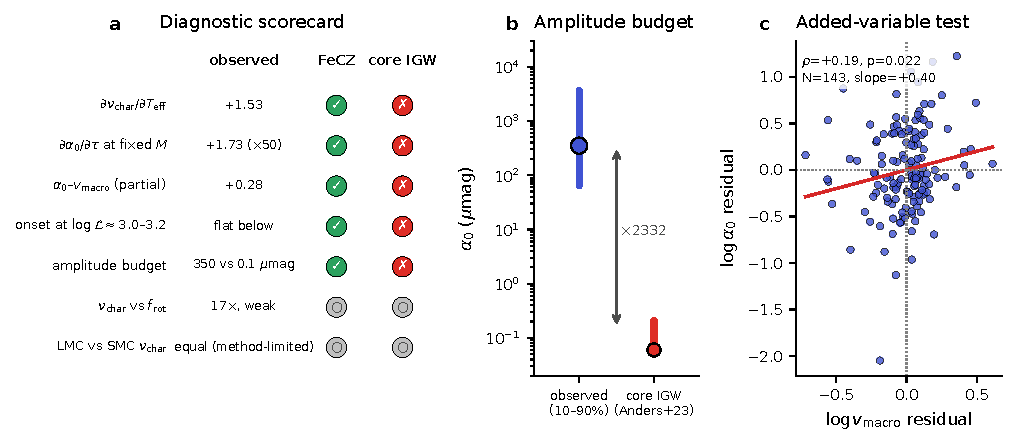
\includegraphics[width=\textwidth]{fig7_theory.pdf}
\caption{Confrontation with theory. (a) Scorecard: the sign or presence of each observed trend against the expectation from sub-surface (FeCZ) convection and from core-excited IGWs; green ticks mark agreement, red crosses disagreement, grey circles tests that do not discriminate. (b) Amplitude budget: the 10--90\% range of observed $\alpha_0$ on the primary sample against the range predicted by 3D simulations of core-excited waves \citep{anders2023}. (c) Added-variable test: the residual of $\log\alpha_0$ against the residual of $\log\vmac$ after both are regressed on $\ell$ and $\teff$.}
\label{fig:theory}
\end{figure*}

\subsection{Sub-surface convection versus core-excited waves}\label{sec:fecz_vs_igw}

Figure~\ref{fig:theory} collects the diagnostics. Five independent trends are each what a sub-surface convection zone predicts and none is what core-excited IGWs predict.

\emph{Coordinates.} FeCZ properties in 1D models are functions of position on the sHRD: the convective flux fraction and velocity increase toward the Eddington limit, i.e.\ with $\ell$, and the turnover time is set by the local scale height and velocity, which at fixed $\ell$ depend on $\teff$ \citep{cantiello2021}. Amplitude following $\ell$ and frequency following $\teff$ is exactly this structure. A single spectrum of core-generated waves filtered by the envelope has no reason to produce two orthogonal coordinates.

\emph{Onset.} The FeCZ is absent below a threshold luminosity and both $\vmac$ (hot stars) and $\alpha_0$ are flat below $\lgL\approx3.0$--3.2, then rise steeply. Core convection exists in every star of the sample and its wave flux varies smoothly with mass.

\emph{Evolution.} Along the main sequence the envelope expands, the FeCZ deepens, and its convective velocity and flux grow; the 50-fold growth of $\alpha_0$ at fixed mass is the signature of a driver that strengthens as the star evolves. Core-excited wave amplitudes at the surface are expected to \emph{decrease} with age as the radiative envelope thickens and radiative damping increases \citep{ratnasingam2020,anders2023}.

\emph{Amplitude budget.} Three-dimensional simulations of waves excited by the convective core predict surface photometric amplitudes of 0.06~$\umag$ for a non-rotating 15~$M_\odot$ star, rising to 0.21~$\umag$ with rotation \citep{anders2023}. The observed 10--90\% range on the primary sample is 64--3600~$\umag$ with median 350~$\umag$; the shortfall is 3--4 orders of magnitude and no plausible correction to the simulations closes it.

\emph{Shared driver.} $\alpha_0$ and $\vmac$ correlate ($\rho=+0.52$), and part of that correlation survives the removal of $\ell$ and $\teff$ (partial $\rho=+0.19$, $p=0.02$; Figure~\ref{fig:theory}c). Most of the raw correlation is shared $\ell$ dependence, but the residual correlation means the two observables respond to the same star-to-star fluctuations in the driver.

The evidence does not exclude a contribution from core-excited waves; it excludes them as the \emph{dominant} source of both phenomena in evolved OB stars.

\subsection{What the factor of six means}\label{sec:factor6}

The amplitude is 5--6 times more sensitive than the velocity to luminosity and to age. If $\vmac$ measures the convective velocity $v_c$ (or the velocity of the waves it launches, which scales with it) and $\alpha_0$ measures a fractional flux perturbation, the natural expectation is $\alpha_0\propto F_c/F_\star\propto\rho v_c^3/\teff^4$, which for fixed $\teff$ and density gives a ratio of 3. The observed ratio of 5--6 requires that the density at the FeCZ, or the efficiency with which turbulent kinetic energy is converted to a photometric signal, also increases along $\ell$ and $\tau$. Both are expected---the FeCZ moves deeper into the envelope and encloses more mass as the star approaches the Eddington limit---but the number is a quantitative target that envelope models must reproduce. Conversely, the ratio is much lower along the mass axis (2.2), because at fixed $\tau$ higher mass raises $\vmac$ strongly ($\partial\log\vmac/\partial\log M=0.60$) while $\alpha_0$ responds less.

\subsection{The sub-onset floor}\label{sec:floor}

Below $\lgL\approx3.0$ the hot IACOB stars have $\vmac\approx16~\kms$ and the few red-noise stars have $\alpha_0\sim30~\umag$, neither zero. The FeCZ picture predicts no signal there at solar metallicity. The residual floor could be the IGW contribution that \citet{anders2023} predict to be small but nonzero, pulsational broadening from coherent modes, or a weaker sub-surface zone (the He~II bump). Because it is metallicity-independent in the IGW case and strongly metallicity-dependent in the FeCZ case, the sub-onset floor at low $Z$ is where a metallicity test would be cleanest.

\subsection{Rotation as a modifier}\label{sec:rot_disc}

The turnover frequency is not the rotation frequency, but rotation leaves a common imprint: all three observables increase weakly with $\vsini$ at fixed $\ell$ and $\teff$. The $\vmac$ dependence, on 832 stars and against the direction of the fitting degeneracy, is secure. In a sub-surface picture rotation can act through the Coriolis force on convection (reducing the turnover time, hence raising $\nuchar$), through the latitude dependence of $\teff$ and $g$, or through mixing that changes the envelope opacity. In the core-IGW picture rotation shifts wave power to lower frequency in the inertial frame \citep{aerts2015}, which is the opposite sign to the observed $\nuchar$--$\vsini$ trend. The rotation term is small enough that it does not affect the maps or the onset and evolution results.

\subsection{The cool side and the supergiant floor}\label{sec:cool_disc}

If $\nuchar$ is a convective turnover frequency, the drop from $\sim$1.5 to $\sim$0.3~$\dinv$ between $\lgT\approx4.3$ and 4.1 marks the point where the FeCZ hands over to the deeper, slower He~II and hydrogen convection zones of cooler envelopes, and the $\sim$0.3~$\dinv$ floor shared by blue and yellow supergiants is the turnover frequency of those zones. The red supergiants do not continue the trend: their distribution is broad and reaches higher frequencies, consistent with granulation on a convective envelope where the relevant scale is the surface pressure scale height rather than a buried zone. The RSG values should be read descriptively rather than within the FeCZ framework.

\subsection{Comparison with envelope models}\label{sec:mesa}

\begin{figure*}
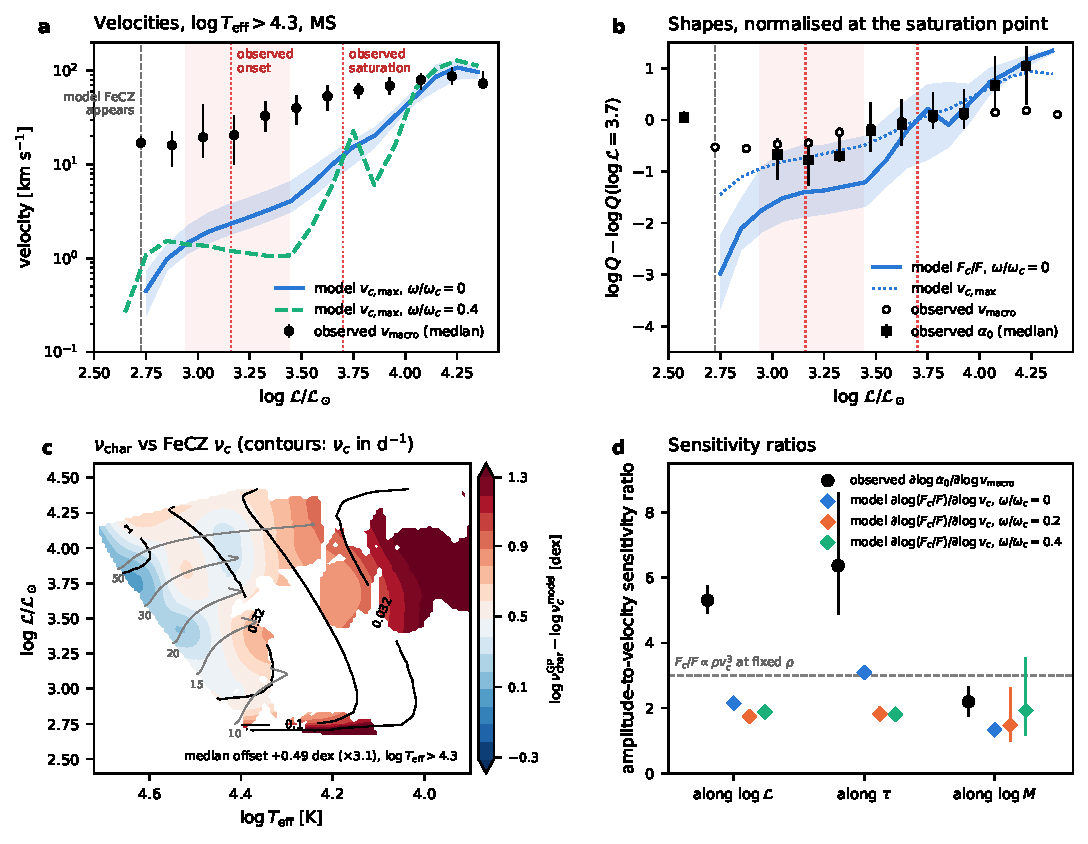
\includegraphics[width=\textwidth]{fig8_mesa.pdf}
\caption{MESA FeCZ models against the observed targets. (a) Maximum convective velocity in the FeCZ of main-sequence models hotter than $\lgT=4.3$ (Galactic, non-rotating: median and 16--84\% band; dashed: $\omega/\omega_c=0.4$) and binned median $\vmac$ of the hot IACOB stars. The shaded band and dotted lines mark the observed onset (3.16 [2.94, 3.44]) and saturation (3.70) hinges; the dashed grey line marks where the FeCZ appears in half of the models. (b) The same model quantities and the observed $\alpha_0$ and $\vmac$, each normalized at $\lgL=3.7$ to compare shapes. (c) Offset between the observed $\nuchar$ GP field (Figure~\ref{fig:gpmaps}; trustworthy cells only) and the FeCZ turnover frequency $\nu_c=1/(2\pi t_c)$ of the models (main sequence and post-main sequence), with $\nu_c$ contours in $\dinv$ and selected tracks. The colour scale is centred on the median offset over $\lgT>4.3$. (d) Amplitude-to-velocity sensitivity ratios along $\ell$, $\tau$, and $M$: observed $\partial\log\alpha_0/\partial\log\vmac$ against the model $\partial\log(F_c/F)/\partial\log v_{c,\max}$ for three rotation rates; the dashed line is the ratio of 3 expected if $F_c/F\propto\rho v_c^3$ at constant density.}
\label{fig:mesa}
\end{figure*}

We confront the three targets with the MESA grid described in Appendix~\ref{app:mesa} (Figure~\ref{fig:mesa}, Table~\ref{tab:mesa}). The primary comparison uses the non-rotating Galactic sub-grid with $\alpha_{\rm MLT}=1.6$ and without MLT++. Model quantities are evaluated on the main sequence, each track weighted equally and sampled uniformly in age, and regressions use the same $\{\ell,\teff\}$ and $\{\tau,\log M\}$ bases and the same domain as the observations.

(i) \emph{Onset.} In the models hotter than $\lgT=4.3$ an FeCZ is present in half of the main-sequence models from $\lgL=2.73$, but it is dynamically negligible there: the median $v_{c,\max}$ exceeds $1~\kms$ only at $\lgL=2.88$ and $3~\kms$ at 3.33, and the convective flux fraction reaches $10^{-3}$ at 3.43. The observed onset, 3.16 [2.94, 3.44], falls where $v_{c,\max}$ crosses 1--$3~\kms$, not where the zone first appears. The 0.4--0.6~dex gap between the appearance of the FeCZ and the observed switch-on is therefore what a velocity (or flux) threshold predicts, and needs no additional physics. The threshold is of order $1~\kms$, an order of magnitude below the $\approx16~\kms$ floor of $\vmac$.

(ii) \emph{Saturation.} The models do not reproduce it. The FeCZ velocity keeps rising steeply through $\lgL=3.7$ ($\partial\log v_{c,\max}/\partial\lgL=+1.56$ below and $+1.72$ above, against $+0.81$ and $+0.29$ for $\vmac$), and it is the flux fraction that flattens ($+3.58$ to $+2.39$), the opposite of the observed pattern. The model velocity reaches the observed $\vmac$ only at $\lgL\approx4.0$--4.2; below that, $\vmac$ exceeds $v_{c,\max}$ by factors of 3 to $\approx15$ (Figure~\ref{fig:mesa}a). A saturation of the photospheric velocity field at $\lgL\approx3.7$ must therefore arise between the FeCZ and the photosphere---for example in the transfer of velocity through the overlying radiative layer---rather than in the convective velocity itself. The flux fraction reaches $10^{-2}$ at $\lgL=3.68$, at the observed saturation point.

(iii) \emph{Sensitivity ratios.} The models reproduce the ordering of the three ratios---largest along $\tau$, smallest along mass---but not their magnitude: $\partial\log(F_c/F)/\partial\log v_{c,\max}=2.15$ [2.01, 2.32] along $\ell$, 3.09 [2.98, 3.22] along $\tau$, and 1.33 [1.16, 1.46] along $M$, against 5.3, 6.4, and 2.2 observed (Figure~\ref{fig:mesa}d). The mechanism proposed in Section~\ref{sec:factor6} does not operate in the models: the density at the FeCZ \emph{decreases} along all three axes ($\partial\log\rho/\partial\lgL=-1.20$, $\partial\log\rho/\partial\tau=-0.38$, $\partial\log\rho/\partial\log M=-1.84$), so $F_c/F$ grows more slowly than $v_c^3$: a $\rho v_c^3$ scaling predicts ratios of 2.2, 2.6, and 2.0, and the model values differ from these by $\le0.7$ because $\teff$ and the zone geometry change as well. Equivalently, the observed quantities respond sub-linearly to the model ones, and to different powers: $\alpha_0\propto(F_c/F)^{0.46\text{--}0.66}$ and $\vmac\propto v_{c,\max}^{0.19\text{--}0.33}$ across the three axes. If $\vmac$ and $\alpha_0$ are set by the FeCZ, the amplitude-to-velocity ratio of 5--6 measures the transfer to the surface, not the zone itself.

\emph{Frequencies.} The FeCZ turnover frequency lies below the observed $\nuchar$ by a factor of 3.1 (median 0.49 dex, 16--84\%: 0.33--0.62 dex, over the trustworthy cells with $\lgT>4.3$), recovering the offset of \citet{cantiello2021}. The offset does not depend on $\ell$ ($+0.06$~dex per dex), and on the main sequence the model reproduces the observed $\teff$ dependence ($\partial\log\nu_c/\partial\lgT=+1.75$ [1.46, 2.00] against $+1.53$) and the near-absence of an $\ell$ dependence ($+0.02$ against $-0.23$). Across the full map, however, the offset grows toward cooler $\teff$ ($-1.1$~dex per dex in $\lgT$; Figure~\ref{fig:mesa}c), because the model $\nu_c$ falls steeply once the FeCZ deepens after the main sequence. At fixed mass the models reproduce the signs of all three evolutionary trends but overshoot the amplitudes: $\partial/\partial\tau=+0.85$ for $\log v_{c,\max}$ and $+2.64$ for $\log F_c/F$ (observed $+0.27$ for $\vmac$ and $+1.73$ for $\alpha_0$), and $-0.12$ [$-0.17$, $-0.06$] for $\log\nu_c$ ($-0.33$ observed).

\emph{Cool side.} The handover interpretation of Section~\ref{sec:cool_disc} is not supported with this definition of the turnover time. In the evolved OB/BSG region ($4.0<\lgT<4.3$, $\lgL>3.6$) the models' FeCZ turns over at 0.018 [0.014, 0.027]~$\dinv$ and the He\,II zone at $7\times10^{-4}~\dinv$, one to three orders of magnitude below the observed 0.27~$\dinv$; in the yellow-supergiant region the FeCZ, He\,II, and H zones give 0.007, 0.010, and 0.014~$\dinv$ against 0.30~$\dinv$ observed.

\emph{Metallicity, rotation, MLT++.} The same analysis on the Magellanic sub-grids moves the model FeCZ appearance to $\lgL=3.18$ (LMC) and 3.68 (SMC), and the $3~\kms$ threshold to 3.73 and 4.18. This is a clean prediction for a homogeneous refit (Section~\ref{sec:metallicity}), but the existing data are already in tension with it: 12 of the 23 SMC stars of \citet{bowman2024} lie below the model FeCZ appearance, and their PSD-proxy amplitudes are indistinguishable from those of the 11 above (Mann--Whitney $p=0.98$). Either the sub-onset driver discussed in Section~\ref{sec:floor} dominates at low $Z$, or the models underpredict the FeCZ at SMC metallicity. Rotation at $\omega/\omega_c=0.2$--0.4 lowers all three sensitivity ratios (1.7--1.9 along $\ell$) and moves the $3~\kms$ threshold to $\lgL\approx3.6$--3.7. MLT++ leaves models below $\approx19\,M_\odot$ unchanged, and hence the onset, but raises the main-sequence median $F_c/F$ by 0.4--1.0~dex at 30--$60\,M_\odot$.

In summary, a single grid with $\alpha_{\rm MLT}=1.6$ reproduces the onset as a threshold effect, the $\teff$ scaling and $\ell$-independence of the turnover frequency up to a constant factor of $\approx3$ on the main sequence, and the sign and ordering of every evolutionary trend and sensitivity ratio. It does not reproduce the saturation of $\vmac$, the magnitude of the sensitivity ratios (low by a factor 1.6--2.5), the cool-side frequencies, or the SMC stars below the model onset. The sub-surface interpretation is therefore supported in its structure but not yet quantitatively; the failures point at the coupling between the FeCZ and the photosphere, which one-dimensional models do not describe.

\subsection{Caveats}\label{sec:caveats}

(1) The Galactic and Magellanic red-noise samples were fitted with different methods (Lorentzian versus GP) that return systematically different $\nuchar$; no cross-galaxy frequency comparison is made here. (2) Published formal uncertainties on the red-noise parameters are unusable and were replaced by a measured study-to-study systematic; that systematic is derived from 24 stars and its dependence on brightness or sector coverage is unknown. (3) Tier-B placement carries a 0.19-dex scatter in $\ell$ and assumes single-star evolution; the calibration sample (33 stars) spans $\lgL=3.2$--4.5. (4) The MIST-based $\tau$ and $M$ assume solar metallicity and $v/v_{\rm crit}=0.4$; the Magellanic stars are placed on the same tracks, which biases their $\tau$ but not their sHRD position. (5) The IACOB sample is magnitude-limited and northern; the red-noise samples are TESS-selected. Neither is complete in any volume, and the sub-onset region is sparsely populated in both. (6) Coherent pulsators, binaries, and magnetic stars are present in the samples and appear among the largest residuals; they were not removed.

\section{Conclusions}\label{sec:conclusions}

From 342 red-noise and 832 macroturbulence measurements placed on a common spectroscopic HR diagram, with evolutionary parameters assigned from MIST tracks:
\begin{enumerate}
\item Red-noise amplitude and macroturbulent velocity are organized by the same sHRD coordinate, $\ell=\teff^4/g$ ($\alpha_0\propto\ell^{1.56}$, $\vmac\propto\ell^{0.29}$ at fixed $\teff$), whereas the characteristic frequency is set by $\teff$ ($\nuchar\propto\teff^{1.5}$) and is independent of $\ell$. The high-frequency slope $\gamma\approx1.9$ is nearly universal.
\item Both $\vmac$ (in stars hotter than $\lgT=4.3$) and $\alpha_0$ switch on at $\lgL\approx3.0$--3.2, $\approx0.6$~dex above the luminosity at which 1D models first develop an iron convection zone, and $\vmac$ saturates at $\lgL\approx3.7$.
\item At fixed mass, $\alpha_0$ grows by a factor of $\sim$50 across the main sequence and $\vmac$ by 1.9$\times$, while $\nuchar$ declines slowly; the amplitude plateaus after the TAMS.
\item The amplitude is 5--6 times more sensitive than the velocity to luminosity and to age, but only $\approx2$ times more sensitive to mass: the two observables share a driver but measure it through different physics.
\item $\nuchar\approx17\,f_{\rm rot}$ with no harmonic pile-up; rotation is not the clock. All three observables nonetheless carry the same weak positive residual dependence on $\vsini$.
\item Every one of these trends is predicted by a deepening, strengthening sub-surface convection zone and none by core-excited gravity waves, whose simulated amplitudes fall 3--4 dex short. Sub-surface convection is the dominant driver of both phenomena in evolved OB stars; a metallicity-independent wave floor below the onset remains possible and untested.
\item On the cool side, $\nuchar$ drops to a $\sim$0.3~$\dinv$ floor shared by blue and yellow supergiants and the red supergiants form a distinct regime.
\end{enumerate}
The onset luminosity, the saturation luminosity, and the axis-dependent amplitude-to-velocity sensitivity ratios are quantitative targets for envelope models; a homogeneous refit of Galactic and Magellanic light curves is the observational step that would unlock the metallicity test.

\begin{acknowledgments}
\todo{Acknowledgments.} This research made use of the VizieR catalogue access tool and the TAP service at CDS, Strasbourg, France; the MESA Isochrones and Stellar Tracks (MIST) grids; and the IACOB spectroscopic database.
\end{acknowledgments}

\facilities{TESS, CoRoT, K2, NOT (FIES), MERCATOR (HERMES), CAO:2.2m (FEROS)}
\software{MESA \citep{paxton2011,paxton2013,paxton2015,paxton2018,paxton2019,jermyn2023}, astropy, numpy, scipy, scikit-learn, pandas, matplotlib}

\appendix

\section{Cross-validation of the red-noise and luminosity inputs}\label{app:validation}

\begin{figure*}
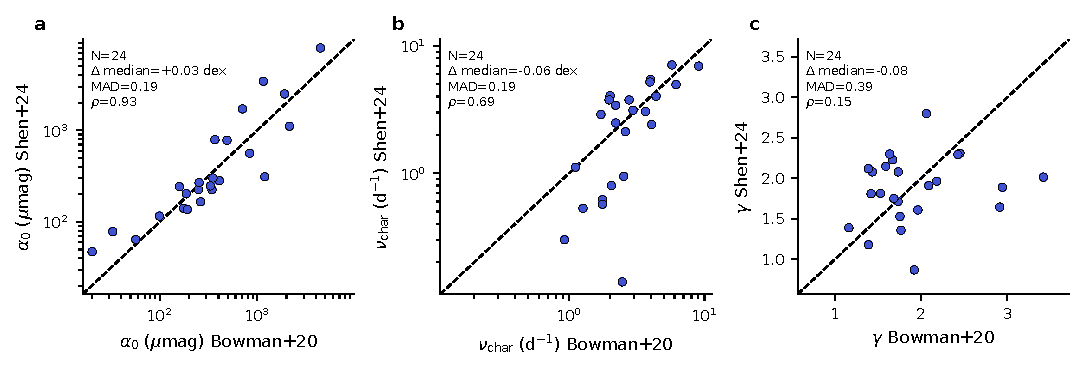
\includegraphics[width=\textwidth]{figA1_overlap.pdf}
\caption{The 24 stars fitted independently by \citet{bowman2020} and \citet{shen2024}: (a) $\alpha_0$, (b) $\nuchar$, (c) $\gamma$. Dashed lines are the identity. The median offset, median absolute deviation about it, and rank correlation are given in each panel; the MAD values are adopted as the per-star systematic uncertainties in Section~\ref{sec:weights}.}
\label{fig:overlap}
\end{figure*}

\begin{figure}
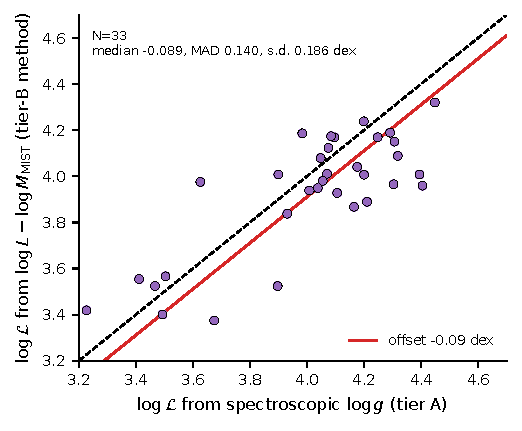
\includegraphics[width=\columnwidth]{figA2_tierB.pdf}
\caption{Calibration of the tier-B placement on the 33 Magellanic stars that have both a spectroscopic $\log g$ (tier A) and a classical luminosity. The red line is the identity shifted by the median offset of $-0.09$~dex, which is applied to all tier-B stars; the scatter of 0.19~dex is propagated into their weights.}
\label{fig:tierB}
\end{figure}

Figure~\ref{fig:overlap} shows the star-by-star comparison of the two Galactic red-noise studies and Figure~\ref{fig:tierB} the tier-B luminosity calibration.

\section{Correlation matrix and machine-readable tables}\label{app:tables}

\begin{figure}
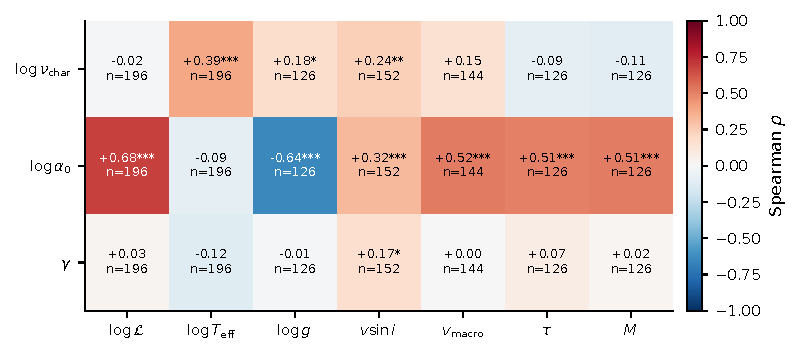
\includegraphics[width=\columnwidth]{figB1_corr.pdf}
\caption{Spearman rank correlations between the red-noise parameters and the stellar parameters on the primary Galactic sample. Asterisks mark $p<0.05$, $0.01$, $0.001$; $n$ is the number of stars with both quantities.}
\label{fig:corr}
\end{figure}

Figure~\ref{fig:corr} gives the full correlation matrix. Two machine-readable tables accompany the paper. \texttt{table\_rednoise\_shrd} lists, for each of the 342 red-noise stars: designation, source sample, placement tier, $\lgT$, $\lgL$, $\alpha_0$ with a flag indicating whether it is $\umag$-compatible, $\nuchar$, $\gamma$, $\vsini$, the MIST-based $\tau$, $\log M$, $\log R$, the projected rotation frequency, and the rotational-modulation candidate flag. \texttt{table\_macroturbulence} lists, for each of the 832 IACOB stars: designation, source, spectral type, $\lgT$, $\lgL$, $\log g$, $\vmac$, $\vsini$, and the same MIST parameters. The fitted GP fields (mean, posterior s.d., trustworthy flag) on both grids are provided as a separate data product.

\section{The MESA model grid}\label{app:mesa}

The models of Section~\ref{sec:mesa} were computed with MESA r26.04.1 \citep{paxton2011,paxton2013,paxton2015,paxton2018,paxton2019,jermyn2023}. The grid comprises 34 initial masses between 5 and $120\,M_\odot$ (steps of $0.2\,M_\odot$ up to 6, $0.5\,M_\odot$ to 8, $1\,M_\odot$ to 25, then 30, 40, 50, 60, 80, 100, and 120) at three metallicities, $Z=0.014$, 0.006, and 0.002 for the Galaxy, LMC, and SMC, each non-rotating and with initial $\omega/\omega_c=0.2$, 0.4, and 0.6 imposed near the ZAMS. Convection follows mixing-length theory with $\alpha_{\rm MLT}=1.6$ and the Schwarzschild criterion. Exponential overshooting ($f=0.014$, $f_0=0.005$) is applied at the top of convective cores and shells. Opacities are the Type-2 OPAL tables with $Z_{\rm base}=Z$ and the \citet{grevesse1998} mixture \todo{confirm mixture: kap default gs98 is used while the inlist comment says Asplund+09}. Mass loss follows the ``Dutch'' combination \citep{glebbeek2009} of \citet{vink2001} for hot stars and de Jager et al.\ (1988) for cool stars, with scaling factor 1. Rotating models include angular-momentum transport and mixing by the Spruit--Tayler dynamo and rotational hydrodynamic instabilities ($f_c=1/30$). MLT++ \citep{paxton2013} is disabled; a non-rotating Galactic sub-grid with MLT++ enabled serves as a differential test. Resolution: \texttt{mesh\_delta\_coeff}\,$=0.3$, $\Delta\lgT$ and $\Delta\log L$ per step limited to 0.005, with gold solver tolerances. Models are evolved to central helium exhaustion.

For every model, sub-surface convective regions are identified from the MESA mixing regions and classified by the temperature at their base as H ($<1.1\times10^4$~K), He\,I ($<3.5\times10^4$~K), He\,II ($<10^5$~K), or Fe ($10^5$--$5\times10^5$~K). For each region we record the maximum and radially averaged MLT convective velocity, the maximum of $L_{\rm conv}/L$, the averaged density and pressure scale height, and the turnover time $t_c=\alpha_{\rm MLT}\bar H_P/\bar v_c$ \citep{cantiello2021}. At the time of writing, 235 \todo{update before submission} of the 408 production tracks have reached central helium exhaustion; all non-rotating Galactic tracks used in the comparison have completed the main sequence except the three most massive (80--$120\,M_\odot$, $X_c\le0.15$). The comparison uses main-sequence models only, except where stated.

\begin{deluxetable*}{lllllcccc}
\tablecaption{Red-noise samples placed on the spectroscopic HR diagram\label{tab:samples}}
\tablehead{\colhead{Source} & \colhead{Galaxy} & \colhead{Fit method} & \colhead{$\alpha_0$ unit} & \colhead{$N$} & \colhead{tier A/B} & \colhead{$N_{\alpha_0}$} & \colhead{$\log T_{\rm eff}$} & \colhead{$\log\mathcal{L}/\mathcal{L}_\odot$}}
\startdata
Bowman et al. (2020) & MW & Lorentzian & $\mu$mag & 70 & 70/0 & 70 & 4.11--4.66 & 2.33--4.33 \\
Shen et al. (2024) & MW & Lorentzian & $\mu$mag & 126 & 126/0 & 126 & 4.44--4.69 & 3.43--4.27 \\
Bowman et al. (2019b) & LMC & Lorentzian & ppm (nominal)$^{\ddagger}$ & 13 & 13/0 & 13$^{\ddagger}$ & 4.25--4.58 & 3.88--4.39 \\
Bowman et al. (2024) & LMC & GP (celerite2) & PSD proxy$^{\dagger}$ & 21 & 17/4 & 0 & 4.16--4.76 & 3.81--4.45 \\
Bowman et al. (2024) & SMC & GP (celerite2) & PSD proxy$^{\dagger}$ & 23 & 15/8 & 0 & 4.28--4.60 & 3.23--4.39 \\
Ma et al. (2024) & LMC & mod. Lorentzian & ppm$^{\ddagger}$ & 13 & 2/11 & 13$^{\ddagger}$ & 4.04--4.29 & 3.28--4.25 \\
Dorn-Wallenstein et al. (2020) & MW & Lorentzian ($\tau$) & ambiguous$^{\dagger}$ & 28 & 0/28 & 0 & 3.66--4.04 & 3.59--4.55 \\
Dorn-Wallenstein et al. (2020) & MW & Lorentzian ($\tau$) & ambiguous$^{\dagger}$ & 48 & 0/48 & 0 & 3.53--3.66 & 3.12--4.58 \\
\enddata
\tablecomments{Tier A: spectroscopic $\log g$ available, $\mathcal{L}=T_{\rm eff}^4/g$ computed directly. Tier B: classical luminosity only; $\mathcal{L}$ from a MIST-track mass (Sect.~\ref{sec:shrd}). $N_{\alpha_0}$: stars whose amplitude enters the sHRD amplitude map and onset test. $^{\ddagger}$ppm amplitudes ($\le0.04$~dex from $\mu$mag) carry an added systematic and are excluded from the scaling-coefficient fits of Table~\ref{tab:fits}, which use the 196 $\mu$mag stars only. $^{\dagger}$Excluded from amplitude analysis (PSD-maximum proxy or unconfirmed unit); used for $\nu_{\rm char}$ and $\gamma$ only.}
\end{deluxetable*}

\begin{deluxetable}{lcc}
\tablecaption{Macroturbulence sources (IACOB family), 832 stars on the sHRD\label{tab:vmac}}
\tablehead{\colhead{Source (priority order)} & \colhead{$N$} & \colhead{median $v_{\rm macro}$ (km\,s$^{-1}$)}}
\startdata
Sim\'on-D\'iaz et al. (2017) & 382 & 41 \\
de Burgos et al. (2024) & 376 & 60 \\
Holgado et al. (2018) & 62 & 76 \\
Burssens et al. (2020) & 12 & 83 \\
\enddata
\tablecomments{When a star appears in several sources, the first in priority order is used. All values are radial--tangential macroturbulent velocities from Fourier-transform plus goodness-of-fit line-profile analyses. Holgado et al. (2018) $T_{\rm eff}$ are tabulated in kK and were converted.}
\end{deluxetable}

\begin{deluxetable*}{lccccc}
\tablecaption{Scaling coefficients (median and 16--84\% bootstrap interval)\label{tab:fits}}
\tablehead{\colhead{Target} & \colhead{$N$} & \colhead{$\partial/\partial\log\mathcal{L}$} & \colhead{$\partial/\partial\log T_{\rm eff}$} & \colhead{$\partial/\partial\log v\sin i$ \,|\, $\partial/\partial\tau$} & \colhead{$\partial/\partial\log v_{\rm macro}$ \,|\, $\partial/\partial\log M$}}
\startdata
\cutinhead{Homogeneous Galactic sample (Bowman et al. 2020 $\cup$ Shen et al. 2024), power-law fits}
$\log\nu_{\rm char}$ & 196 & $-0.23^{+0.09}_{-0.09}$ & $+1.53^{+0.35}_{-0.33}$ & \nodata & \nodata \\
$\log\nu_{\rm char}$ & 152 & $-0.26^{+0.09}_{-0.09}$ & $+1.20^{+0.35}_{-0.35}$ & $+0.34^{+0.09}_{-0.09}$ & \nodata \\
$\log\alpha_0$ & 196 & $+1.56^{+0.12}_{-0.13}$ & $-3.16^{+0.62}_{-0.66}$ & \nodata & \nodata \\
$\log\alpha_0$ & 144 & $+1.43^{+0.15}_{-0.16}$ & $-3.04^{+0.73}_{-0.77}$ & \nodata & $+0.28^{+0.18}_{-0.13}$ \\
\cutinhead{Main-sequence stars, track-based $\tau$ and $M$: $\log(\cdot)=a\,\tau+b\,\log M$}
$\log\alpha_0$ & 190 & \nodata & \nodata & $+1.73^{+0.18}_{-0.16}$$^{\,(\tau)}$ & $+1.32^{+0.20}_{-0.21}$$^{\,(\log M)}$ \\
$\log\nu_{\rm char}$ & 221 & \nodata & \nodata & $-0.33^{+0.14}_{-0.15}$$^{\,(\tau)}$ & $+0.12^{+0.09}_{-0.09}$$^{\,(\log M)}$ \\
$\log v_{\rm macro}$ & 562 & \nodata & \nodata & $+0.27^{+0.05}_{-0.05}$$^{\,(\tau)}$ & $+0.60^{+0.03}_{-0.03}$$^{\,(\log M)}$ \\
\enddata
\tablecomments{Upper block: linear models in log space on the $\mu$mag-matched Galactic sample; $\mathcal{L}$, $T_{\rm eff}$ and $\log g$ are algebraically degenerate so only the $\{\mathcal{L},T_{\rm eff}\}$ basis is used. Lower block: separate two-predictor model on main-sequence stars ($\tau<1$) with $\tau$ and $M$ assigned from MIST tracks (Sect.~\ref{sec:evol}); the last two columns give the $\tau$ and $\log M$ slopes.}
\end{deluxetable*}

\begin{deluxetable*}{lcccccccc}
\tablecaption{Broken-power-law test for a luminosity onset ($T_{\rm eff}$-controlled)\label{tab:onset}}
\tablehead{\colhead{Quantity} & \colhead{$N$} & \colhead{single slope} & \colhead{hinge $\log\mathcal{L}$ [16--84\%]} & \colhead{slope below} & \colhead{slope above} & \colhead{$N_{\rm below}$} & \colhead{$\Delta$BIC} & \colhead{break?}}
\startdata
$\alpha_0$ (OB) & 222 & +1.27 & 3.16 [2.94, 3.44] & -0.02 & +1.66 & 19 & +16.3 & yes \\
$\nu_{\rm char}$ (OB) & 271 & -0.32 & 4.02 [2.96, 4.14] & -0.22 & -0.93 & 171 & -0.6 & no \\
$v_{\rm macro}$ (all) & 832 & +0.29 & 2.96 [2.90, 3.10] & -0.18 & +0.44 & 162 & +95.5 & yes \\
$v_{\rm macro}$ ($\log T_{\rm eff}>4.3$) & 579 & +0.52 & 3.80 [3.70, 3.84] & +0.66 & +0.27 & 245 & +14.9 & yes \\
$v_{\rm macro}$ ($4.0<\log T_{\rm eff}\le4.3$) & 253 & +0.16 & 2.78 [2.68, 3.08] & -0.08 & +0.23 & 125 & +4.8 & no \\
\enddata
\tablecomments{Model: $\log(\cdot)=c_0+c_1(\log\mathcal{L}-h)+c_2\max(0,\log\mathcal{L}-h)+c_3\log T_{\rm eff}$; hinge $h$ scanned on a 0.02-dex grid, bootstrap interval from 300 resamples. $\Delta{\rm BIC}=$ BIC(single) $-$ BIC(broken); a break is claimed for $\Delta{\rm BIC}>6$ with the hinge away from the grid edge. For the hot subsample a second hinge at $\log\mathcal{L}=3.70$ is favoured over one hinge by $\Delta{\rm BIC}=17.5$ (slopes $+0.37/+0.81/+0.29$).}
\end{deluxetable*}

\begin{deluxetable}{lcccc}
\tablecaption{Red-noise parameters by HRD region\label{tab:regions}}
\tablehead{\colhead{Region} & \colhead{$N$} & \colhead{$\nu_{\rm char}$ (d$^{-1}$)} & \colhead{$N_\gamma$} & \colhead{$\gamma$}}
\startdata
hot OB ($\log T_{\rm eff}\ge4.3$) & 235 & 1.47 [0.45, 3.80] & 193 & 1.91 [1.43, 2.45] \\
evolved OB/BSG ($4.0$--$4.3$, $\log\mathcal{L}>3.6$) & 22 & 0.27 [0.20, 0.46] & 20 & 2.58 [2.09, 3.39] \\
YSG ($3.75$--$4.0$) & 20 & 0.30 [0.17, 0.50] & 20 & 1.63 [1.38, 1.89] \\
RSG ($\log T_{\rm eff}<3.75$) & 51 & 0.59 [0.33, 2.33] & 51 & 1.72 [1.48, 2.27] \\
\enddata
\tablecomments{Median and 16--84\% range. Bowman et al. (2024) $\nu_{\rm char}$ values are GP-based and systematically offset from Lorentzian fits (Bowman \& Dorn-Wallenstein 2022); they enter the hot-OB and evolved rows.}
\end{deluxetable}

% Generated from analysis_mesa/data/mesa_{onset,slopes,ratios,nuc_offset,coolside}.csv
% (compare_obs.py). Model: MW, omega/omega_c = 0, alpha_MLT = 1.6, no MLT++; MS models.
\begin{deluxetable*}{llll}
\tabletypesize{\footnotesize}
\tablewidth{0pt}
\tablecaption{Observed targets and the MESA FeCZ models\label{tab:mesa}}
\tablehead{\colhead{Target} & \colhead{Observed} & \colhead{Model ($Z=0.014$, $\omega/\omega_c=0$)} & \colhead{Outcome}}
\startdata
\multicolumn{4}{l}{\emph{(i) Onset}}\\
\quad $\lgL$ of onset ($\lgT>4.3$) & 3.16 [2.94, 3.44] & FeCZ appears 2.73 & threshold at \\
\quad $\lgL$ where $v_{c,\max}>1$, $3~\kms$ & \nodata & 2.88, 3.33 & $v_c\approx1$--$3~\kms$ \\
\quad $\lgL$ where $F_c/F>10^{-3}$, $10^{-2}$ & \nodata & 3.43, 3.68 & \\
\multicolumn{4}{l}{\emph{(ii) Saturation at $\lgL=3.70$}}\\
\quad velocity slope in $\ell$, below $\to$ above & $+0.81\to+0.29$ ($\vmac$) & $+1.56\to+1.72$ ($v_{c,\max}$) & not reproduced \\
\quad amplitude slope in $\ell$ & $+1.66$ above ($\alpha_0$) & $+3.58\to+2.39$ ($F_c/F$) & \\
\multicolumn{4}{l}{\emph{(iii) Amplitude-to-velocity sensitivity ratio}}\\
\quad along $\lgL$ & 5.3 [4.9, 5.8] & 2.15 [2.01, 2.32] & order reproduced, \\
\quad along $\tau$ & 6.4 [4.9, 8.6] & 3.09 [2.98, 3.22] & low by $\times$1.6--2.5 \\
\quad along $\log M$ & 2.2 [1.8, 2.7] & 1.33 [1.16, 1.46] & \\
\multicolumn{4}{l}{\emph{Secondary}}\\
\quad $\nuchar/\nu_c$ ($\lgT>4.3$) & \nodata & $\times3.1$ (0.49 [0.33, 0.62] dex) & flat in $\ell$, not in $\teff$ \\
\quad $\nu$ slopes in $\teff$, $\ell$ & $+1.53$, $-0.23$ & $+1.75$ [1.46, 2.00], $+0.02$ & $\teff$ slope matches \\
\quad $\tau$ slopes: velocity, amplitude, $\nu$ & $+0.27$, $+1.73$, $-0.33$ & $+0.85$, $+2.64$, $-0.12$ & signs reproduced \\
\quad $\nu$, evolved OB/BSG [$\dinv$] & 0.27 [0.20, 0.46] & 0.018 (FeCZ), $7\times10^{-4}$ (He\,II) & not reproduced \\
\enddata
\tablecomments{Model values are medians or regression coefficients over main-sequence models of the non-rotating Galactic sub-grid, each track weighted equally and sampled uniformly in main-sequence age; intervals are 16--84\% from a bootstrap over tracks. Onset luminosities are the centres of the 0.05-dex bins where the median model first exceeds the stated value. $\nu_c=1/(2\pi t_c)$ with $t_c=\alpha_{\rm MLT}H_P/v_c$ averaged over the zone. Regressions use the $\{\ell,\teff\}$ basis over the domain of the primary sample ($\lgL=2.75$--4.21, $\lgT=4.23$--4.61) or $\tau+\log M$ over $\log M=1.01$--1.70.}
\end{deluxetable*}


\bibliographystyle{aasjournal}
\bibliography{refs}

\end{document}
